\let\negmedspace\undefined
\let\negthickspace\undefined
\documentclass[journal,12pt,twocolumn]{IEEEtran}

\usepackage{cite}
\usepackage{amsmath,amssymb,amsfonts,amsthm}
\usepackage{algorithmic}
\usepackage{graphicx}
\usepackage{textcomp}
\usepackage{xcolor}
\usepackage{txfonts}
\usepackage{listings}
\usepackage{enumitem}
\usepackage{mathtools}
\usepackage{gensymb}
\usepackage[breaklinks=true]{hyperref}
\usepackage{tkz-euclide} % loads  TikZ and tkz-base
\usepackage{listings}
\usepackage{circuitikz}
\usepackage{graphicx}

%\newcounter{MYtempeqncnt}
\DeclareMathOperator*{\Res}{Res}
%\renewcommand{\baselinestretch}{2}
\renewcommand\thesection{\arabic{section}}
\renewcommand\thesubsection{\thesection.\arabic{subsection}}
\renewcommand\thesubsubsection{\thesubsection.\arabic{subsubsection}}

\renewcommand\thesectiondis{\arabic{section}}
\renewcommand\thesubsectiondis{\thesectiondis.\arabic{subsection}}
\renewcommand\thesubsubsectiondis{\thesubsectiondis.\arabic{subsubsection}}

% correct bad hyphenation here
\hyphenation{op-tical net-works semi-conduc-tor}
\def\inputGnumericTable{}                                 %%

\lstset{
	frame=single,
	breaklines=true,
	columns=fullflexible
}



\newtheorem{theorem}{Theorem}[section]
\newtheorem{problem}{Problem}
\newtheorem{proposition}{Proposition}[section]
\newtheorem{lemma}{Lemma}[section]
\newtheorem{corollary}[theorem]{Corollary}
\newtheorem{example}{Example}[section]
\newtheorem{definition}[problem]{Definition}
\newcommand{\BEQA}{\begin{eqnarray}}
	\newcommand{\EEQA}{\end{eqnarray}}
\newcommand{\define}{\stackrel{\triangle}{=}}

\bibliographystyle{IEEEtran}
%\bibliographystyle{ieeetr}


\providecommand{\mbf}{\mathbf}
\providecommand{\pr}[1]{\ensuremath{\Pr\left(#1\right)}}
\providecommand{\qfunc}[1]{\ensuremath{Q\left(#1\right)}}
\providecommand{\sbrak}[1]{\ensuremath{{}\left[#1\right]}}
\providecommand{\lsbrak}[1]{\ensuremath{{}\left[#1\right.}}
\providecommand{\rsbrak}[1]{\ensuremath{{}\left.#1\right]}}
\providecommand{\brak}[1]{\ensuremath{\left(#1\right)}}
\providecommand{\lbrak}[1]{\ensuremath{\left(#1\right.}}
\providecommand{\rbrak}[1]{\ensuremath{\left.#1\right)}}
\providecommand{\cbrak}[1]{\ensuremath{\left\{#1\right\}}}
\providecommand{\lcbrak}[1]{\ensuremath{\left\{#1\right.}}
\providecommand{\rcbrak}[1]{\ensuremath{\left.#1\right\}}}
\theoremstyle{remark}
\newtheorem{rem}{Remark}
\newcommand{\sgn}{\mathop{\mathrm{sgn}}}
\providecommand{\abs}[1]{\left\vert#1\right\vert}
\providecommand{\res}[1]{\Res\displaylimits_{#1}}
\providecommand{\norm}[1]{\left\lVert#1\right\rVert}
%\providecommand{\norm}[1]{\lVert#1\rVert}
\providecommand{\mtx}[1]{\mathbf{#1}}
\providecommand{\mean}[1]{E\left[ #1 \right]}
\providecommand{\fourier}{\overset{\mathcal{F}}{ \rightleftharpoons}}
%\providecommand{\hilbert}{\overset{\mathcal{H}}{ \rightleftharpoons}}
\providecommand{\system}{\overset{\mathcal{H}}{ \longleftrightarrow}}
%\newcommand{\solution}[2]{\textbf{Solution:}{#1}}
\newcommand{\solution}{\noindent \textbf{Solution: }}
\newcommand{\cosec}{\,\text{cosec}\,}
\providecommand{\dec}[2]{\ensuremath{\overset{#1}{\underset{#2}{\gtrless}}}}
\newcommand{\myvec}[1]{\ensuremath{\begin{pmatrix}#1\end{pmatrix}}}
\newcommand{\mydet}[1]{\ensuremath{\begin{vmatrix}#1\end{vmatrix}}}
\renewcommand{\abstractname}{Question}

\let\vec\mathbf

	
	\vspace{3cm}
	
	


\newcommand{\permcomb}[4][0mu]{{{}^{#3}\mkern#1#2_{#4}}}
\newcommand{\comb}[1][-1mu]{\permcomb[#1]{C}}

%\IEEEpeerreviewmaketitle

\newcommand \tab [1][1cm]{\hspace*{#1}}
%\newcommand{\Var}{$\sigma ^2$}
\usepackage{amssymb}
\usepackage{amsmath}
\title{
	
\title{NCERT Physics 12.7 Q19}
\author{EE23BTECH11212 - MANUGUNTA MEGHANA SAI$^{*}$% <-this % stops a space
}


}
\begin{document}

\maketitle

\textbf{Question:} 
Suppose the circuit in Exercise 7.18 has a resistance of 15 Ω. Obtain the average power transferred to each element of the circuit, and the total power absorbed.\\
\\

\begin{figure}[h]
	\centering
	    \begin{circuitikz}
		% Draw the components
		\draw (0,0) to[V, v=$230\,V$, f=$50\,Hz$] (0,3)
		to[R, l=$15\,\Omega$] (3,3)
		to[L, l=$80\,mH$] (6,3)
		to[C, l=$60\,\mu F$] (6,0)
		-- (0,0);
     \end{circuitikz}
	

	\caption{LCR Circuit}
	\label{fig:2}
\end{figure}
     
\textbf{Solution: }
In Exercise 7.18, the following information is provided:
 
 

 \begin{table}[h]
 	\centering
 	\resizebox{6 cm}{!}{
 		\begin{tabular}{c|c|c}
	\hline
	Description & Symbol & Value\\
	\hline
	Inductance & L &  $80\, \text{mH}$\\
	Capacitance & C &  $60\, \mu\text{F}$\\
	Resistance & R &  $15\, \Omega$\\
	Voltage & V & $230\, \text{V}$\\
	Frequecny & f & $50\, \text{Hz}$\\
	\hline
\end{tabular}
 	}
 	\vspace{6 pt}
 	\caption{Impedences}
 	\label{tab:my_label} 
 \end{table}
 

Angular frequency of signal, $\omega$ = 2$\pi$$f$ = 2$\pi \cdot \left(50\right)$ 

= $100\pi$
 
 
 
 The elements are connected in series to each other. Hence the impedence $Z$ is givan as :
 \
 \begin{align}
 Z &= \sqrt{R^2 + \left(\omega\cdot L - \frac{1}{\omega\cdot C}\right)^2}
 \\&= \sqrt{15^2 + \left(100\pi\cdot\brak{80 \times 10^{-3}} - \frac{1}{100\pi \times 60 \times 10^{-6}}\right)^2}
 \\&= \sqrt{15^2 + \left(25.12 - 53.08\right)^2}
 \\&=31.728\hspace{0.2cm}\ohm
\end{align}	



Current flowing through the circuit $I$ is :

\begin{align}
	I&=\frac{V}{Z}=\frac{230}{31.728}
	\\&=7.25\hspace{0.2cm}A
\end{align}

Average power transferred to resistance is given by :
\begin{align}
	P_R &= I^2\cdot R = \brak{7.25}^2 \times 15
	\\&=788.44\hspace{0.2cm}W
\end{align}

Average power transferred to the capacitor, $P_C$ = Average power transferred to the inductor, $P_L$ = 0

Total power absorbed by circuit:

\begin{align}
	&= P_R + P_C + P_L
	\\&= 788.44 + 0 + 0
	\\&= 788.44\hspace{0.2cm}W
\end{align}

Total power absorbed by circuit is 788.44\hspace{0.01cm}W

\vspace{1cm}

\textbf{Function \(H(s)\):}


\begin{equation}
	V(s) = R I(s) + sL I(s) + \dfrac{1}{sC} I(s)
\end{equation}


\begin{equation}
	\Rightarrow V(s) = I(s)\left(R + Ls + \dfrac{1}{sC}\right)
\end{equation}

\begin{equation}
	\Rightarrow I(s) = \dfrac{V(s)}{\left(R + Ls + \dfrac{1}{sC}\right)} \label{eq: 4}
\end{equation}

\begin{equation}
	H(s) = \dfrac{V(s)}{I(s)}
\end{equation}

\begin{equation}
	H(s) = R + sL + \dfrac{1}{sC}
\end{equation}

\begin{equation}
	\Rightarrow H(j\omega) = R + j\omega L + \dfrac{1}{j\omega C}
\end{equation}

\begin{equation}
	\Rightarrow \lvert H(j\omega) \rvert = \sqrt{R^2 + \left(\omega L - \dfrac{1}{\omega C}\right)^2}
\end{equation}


\begin{figure}
	\centering
	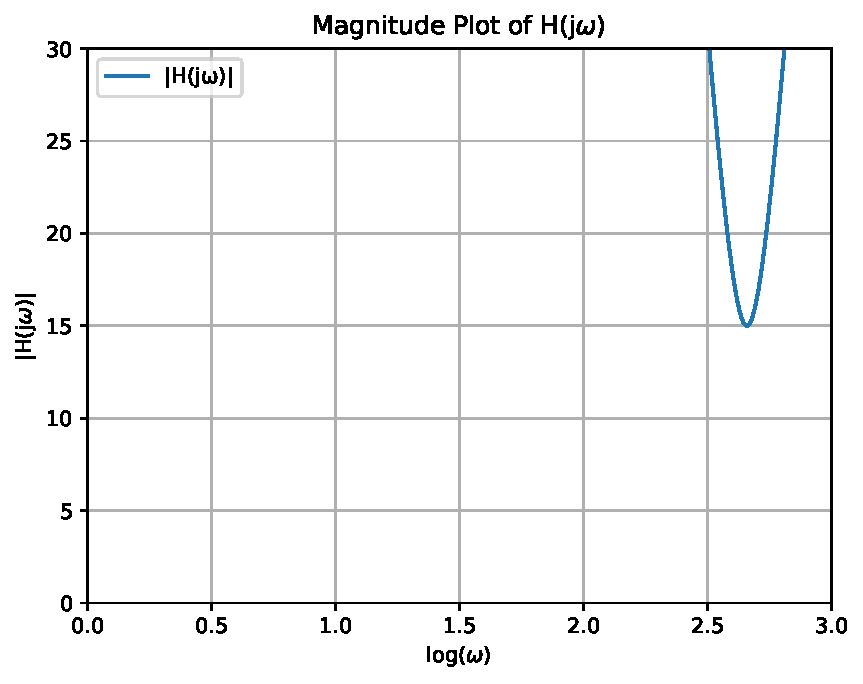
\includegraphics[width=0.8\textwidth]{figs/magnitude_plot.pdf}
	\caption{Absolute value of $H(j\omega)$ for RLC Circuit}
	\label{fig:magnitude_plot}
\end{figure}

 
\end{document}

